\section{Segunda captura y análisis}

\subsection{Explicación del experimento}
\par En este segundo experimento vamos a analizar la ruta desde GBA hasta la \textbf{University of Technology [utech.edu.jm]}, ubicada en Kingston, Jamaica. Dado que Jamaica es una isla, la ruta debe tener al menos un salto por agua.

\subsection{Resultados obtenidos}

\begin{figure}[h!]
  \begin{subfigure}[b]{.5\textwidth}
    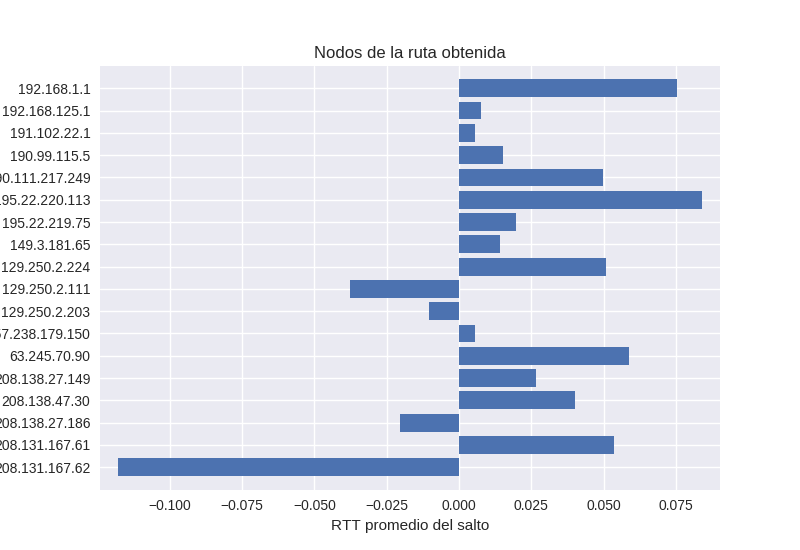
\includegraphics[width=\textwidth]{Imagenes/jamaica_rtts.png}
  \end{subfigure}
  \label{fig:jamaica_rtts}
  \caption{Tiempo del salto entre cada nodo y su nodo previo, para cada nodo identificado en el camino al host utech.edu.jm}
\end{figure}

\par En el gráfico correspondiente a la figura 4 se puede observar que los promedios positivos no varían mucho, en particular la media muestral de todos los datos (negativos o positivos) es 0.025796904867776 mientras que la varianza es 0.001129809044593, que son algunos órdenes de magnitud menos. Que la varianza sea tan pequeña nos quiere decir que los datos no presentan una gran dispersión y, por ende, no es muy probable que haya outliers.

\begin{figure}[h!]
  \begin{subfigure}[b]{.5\textwidth}
    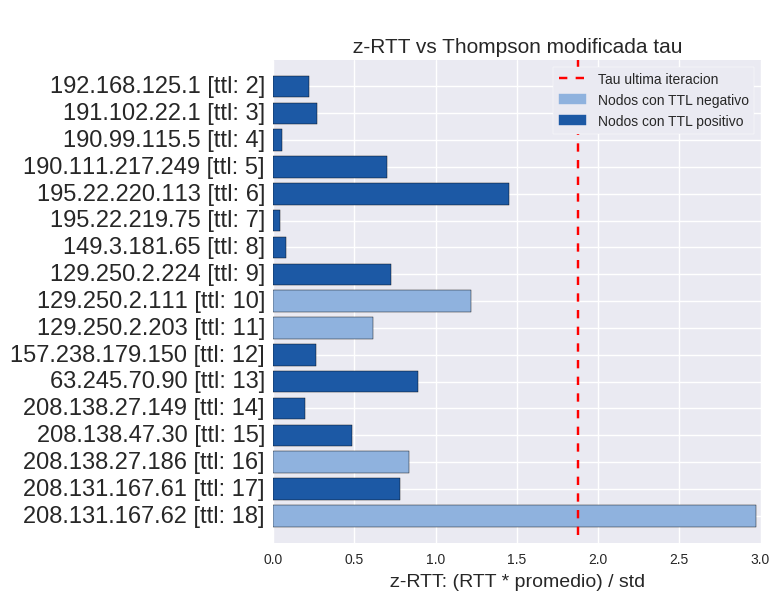
\includegraphics[width=\textwidth]{Imagenes/jamaica_zrtts.png}
  \end{subfigure}
  \label{fig:jamaica_zrtts}
  \caption{zRTT de los nodos del camino al host utech.edu.jm comparado con el umbral establecido por el valor de Thompson modificado.}
\end{figure}

\begin{figure*}[ht]
  \hspace*{-0.4cm}
  \begin{subfigure}[b]{.60\textwidth}
    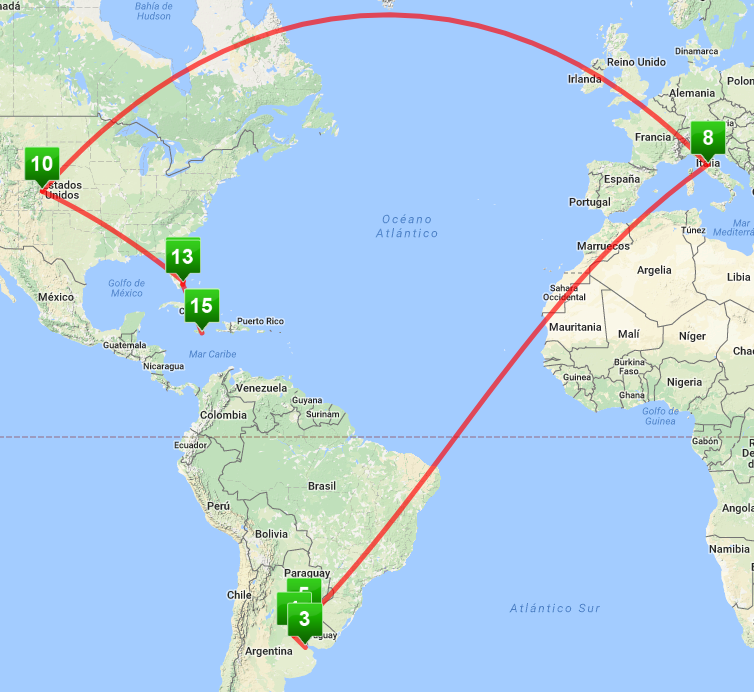
\includegraphics[width=\textwidth]{Imagenes/jamaica_map.png}
    \label{fig:jamaica_map}
    \caption{Mapa que muestra la unión de los nodos que forman el camino.}
  \end{subfigure}
  \begin{subfigure}[b]{.39\textwidth}
    \footnotesize
    \begin{tabular}{ l l l }
      \hline
      \textbf{TTL} & \textbf{IP} &  \textbf{País - Ciudad} \\ \hline
      1 & 192.168.1.1 &\\ \hline
      2 & 192.168.125.1 &\\ \hline
      3 & 191.102.22.1 & Argentina - Morón\\ \hline
      4 & 190.99.115.5 & Argentina - Rosario\\ \hline
      5 & 190.111.217.249 & Argentina - Entre Ríos\\ \hline
      \rowcolor[RGB]{196,214,255}
      6 & 195.22.220.113 & Italia\\ \hline
      7 & 195.22.219.75 & Italia\\ \hline
      8 & 149.3.181.65 & Italia\\ \hline
      \rowcolor[RGB]{196,214,255}
      9 & 129.250.2.224 & Estados Unidos - Colorado \\ \hline
      10 & 129.250.2.111 & Estados Unidos - Colorado\\ \hline
      11 & 129.250.2.203 & Estados Unidos - Colorado\\ \hline
      12 & 157.238.179.150 & Estados Unidos - Florida\\ \hline
      13 & 63.245.70.90 & Estados Unidos - Florida\\ \hline
      \rowcolor[RGB]{196,214,255}
      14 & 208.138.27.149 & Jamaica - Kinsgton\\ \hline
      15 & 208.138.47.30 & Jamaica - Kingston\\ \hline
      16 & 208.138.27.186 & Jamaica - Kingston\\ \hline
      17 & 208.131.167.61 & Jamaica - Kingston\\ \hline
      18 & 208.131.167.62 & Jamaica - Kingston \\ \hline
      \hline
    \end{tabular}
    \label{fig:jamaica_list}
    \caption{Listado de nodos: TTL, IP y ubicación geográfica.}
  \end{subfigure}
  \caption{Nodos pertenecientes al camino al host utech.edu.jm.}
\end{figure*}

\par Luego, ejecutamos nuestro algoritmo de detección de outliers y, como era de esperar, no se obtuvieron outliers. En la tabla en la que exhibimos la ruta se muestran en azul los tres saltos intercontinentales que realizaron los paquetes hasta llegar a la University of Technology. Esto es particularmente llamativo dado que según el planisferio de enlaces intercontinentales\footnote{Mapa de enlaces intercontinentales: http://www.muycomputer.com/wp-content/uploads/2011/09/mundo.86i.cyp3mivcag.jpeg} hay por lo menos dos caminos posibles cuya longitud es mucho menor (un enlace desde Chile hasta Panamá y luego desde Panamá hasta Jamaica y la otra opción es ir por la costa de Brasil para luego acceder a Jamaica). La explicación que le pudimos encontrar a este comportamiento es que al haber muchísimos enlaces entre Europa y Estados Unidos la red prefiere ir hacia Europa para luego tener varias opciones para regresar al continente americano.
\par En este caso todos los hops respondieron nuestros mensajes. La ruta, a nuestro criterio, no es tan larga, pero tiene demasiados saltos intercontinentales.
